\documentclass{standalone}
\usepackage{graphicx}
\graphicspath{./img/ }

\begin{document}

\section*{5.1\hspace{0.3 cm} The Frontend}
\addcontentsline{toc}{section}{5.1\hspace{0.3 cm} The Frontend} \vspace{0.3cm}

\hspace{0.5cm} The implementation of this project's one part is frontend other one described later. In frontend we used ReactJS. React (also known as React.js or ReactJS) is an open-source, front end, JavaScript library for building user interfaces or UI components. It is maintained by Facebook and a community of individual developers and companies.  React can be used as a base in the development of single-page or mobile applications.\vspace{1cm}

\subsection*{5.1.1\hspace{0.3 cm} The Frontend UI and Coding Template}
\addcontentsline{toc}{subsection}{5.1.1\hspace{0.3 cm} The Frontend UI and Coding Template} \vspace{0.3cm}

\newpage
\vfill

\begin{figure}

\includegraphics{./img/img1.png} 
\caption{SignIn UI}
 \label{fig:sign}
\end{figure}

\begin{figure}
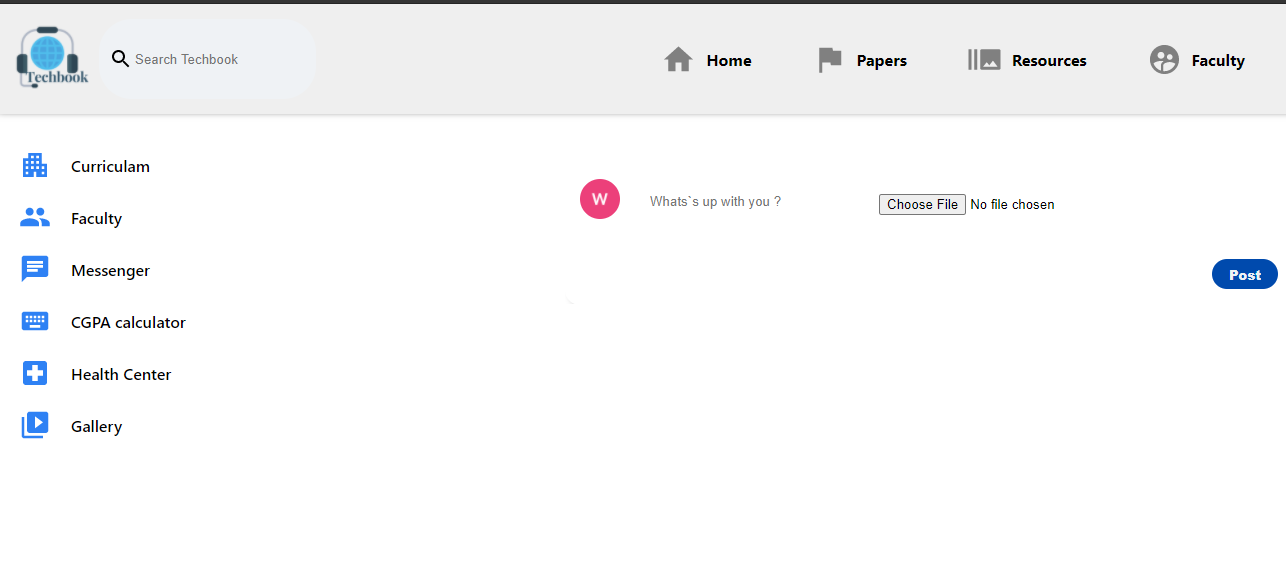
\includegraphics[scale=0.4]{./img/img2.png}
\caption{Home UI}
 \label{fig:home}
\end{figure}

\begin{figure}
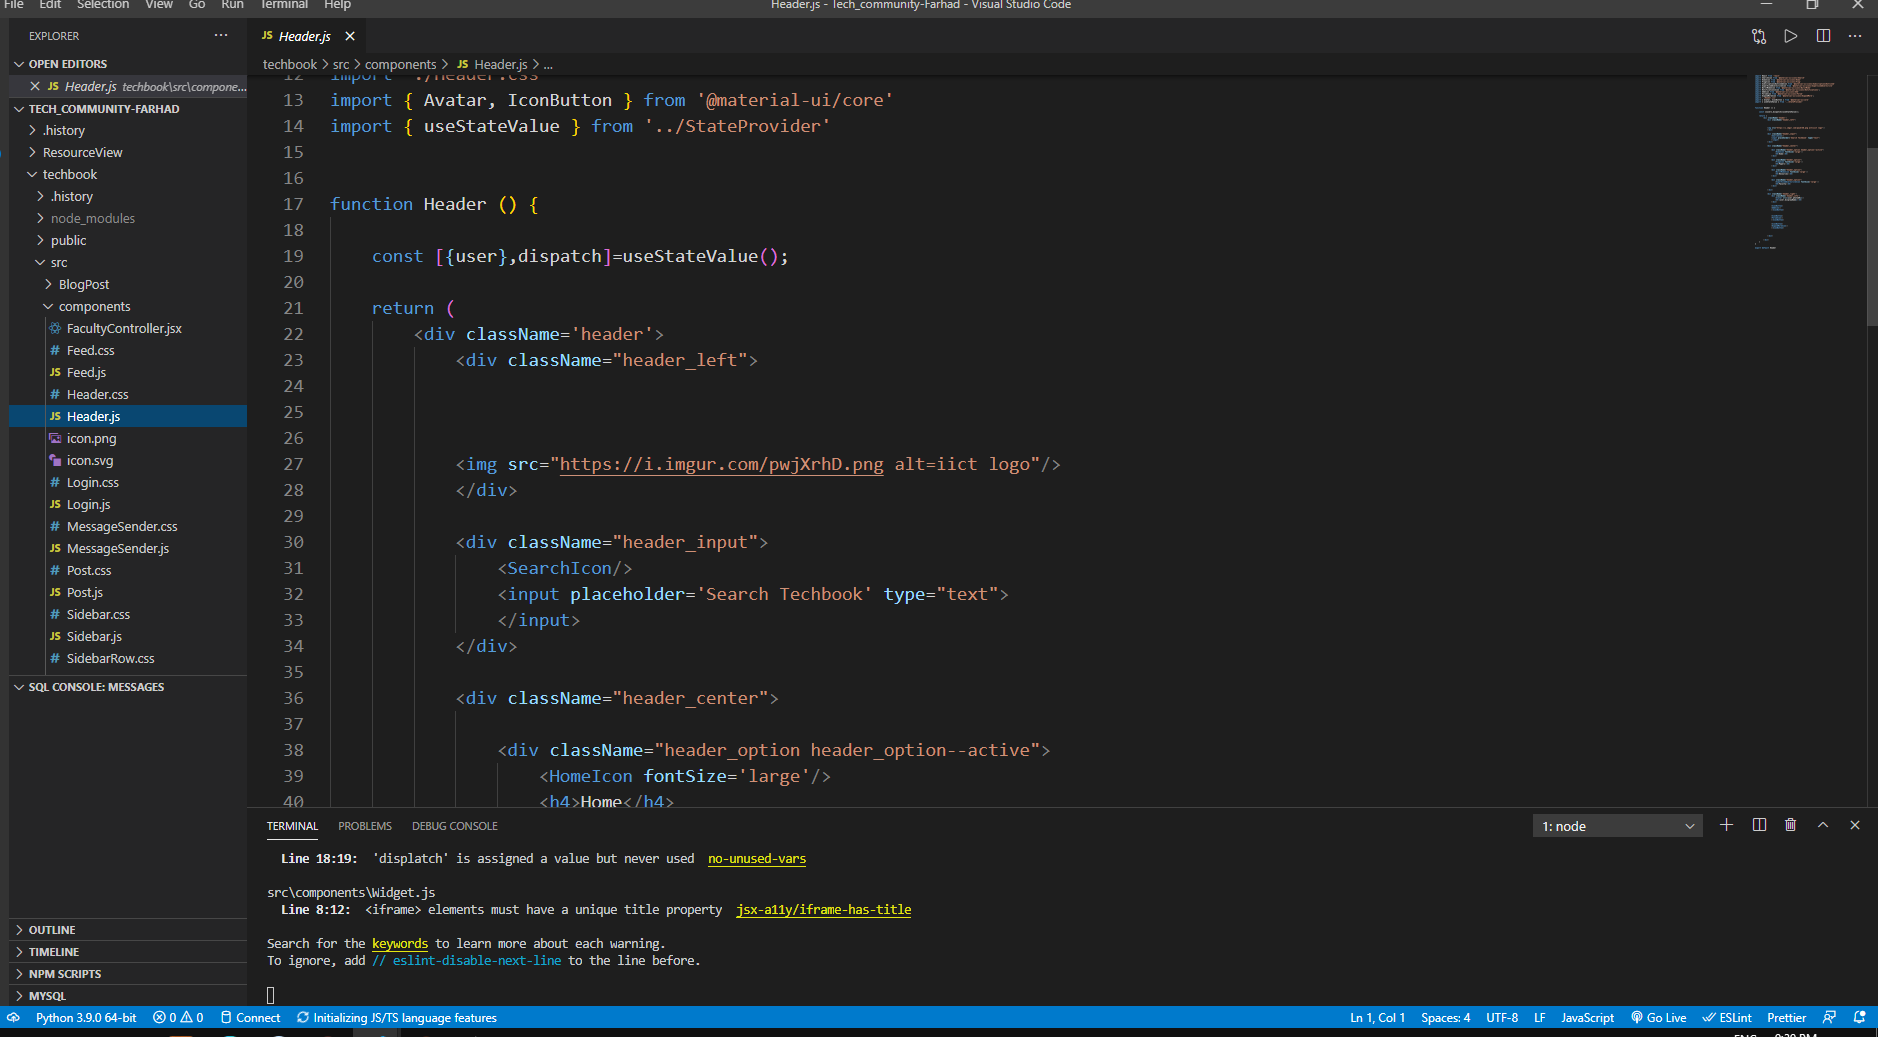
\includegraphics[scale=0.3]{./img/img3.png}\\[2cm]
\caption{Frontend Coding Template}
\label{fig:Frontend}
\end{figure}

\clearpage
\vfill


\section*{5.2\hspace{0.3 cm} The Backend}
\addcontentsline{toc}{section}{5.2\hspace{0.3 cm} The Backend} \vspace{0.3cm}

\hspace{0.5cm} The other part of this project is backend and database. In backend we used NodeJS and ExpressJS(Node framework).
Node.js is primarily used for non-blocking, event-driven servers, due to its single-threaded nature. It's used for traditional web sites and back-end API services, but was designed with real-time, push-based architectures in mind.\\[0.8cm]


\subsection*{5.2.1\hspace{0.3 cm} The Backend Coding Template and DB}
\addcontentsline{toc}{subsection}{5.2.1\hspace{0.3 cm} The Backend Coding Template and DB} \vspace{0.8cm}

\hspace{0.5cm} In database we used MongoDB Database. MongoDB is a document database in which one collection holds different documents. Number of fields, content and size of the document can differ from one document to another.It is easy to scale.Deep query-ability. MongoDB supports dynamic queries on documents using a document-based query language that's nearly as powerful as SQL.\\[0.8cm]

\subsection*{5.2.2\hspace{0.3 cm} Internal Api}
\addcontentsline{toc}{subsection}{5.2.2\hspace{0.3 cm} Internal Api} \vspace{0.8cm}

\hspace{0.5cm} We also used internal api for sharing data. One of the key advantages of internal APIs is that it provides a great deal of flexibility. Data is not tied to resources or methods. We uses this type of API among the different internal teams to be able to improve its sharing data flexibility.

\newpage
\vfill
\begin{figure}
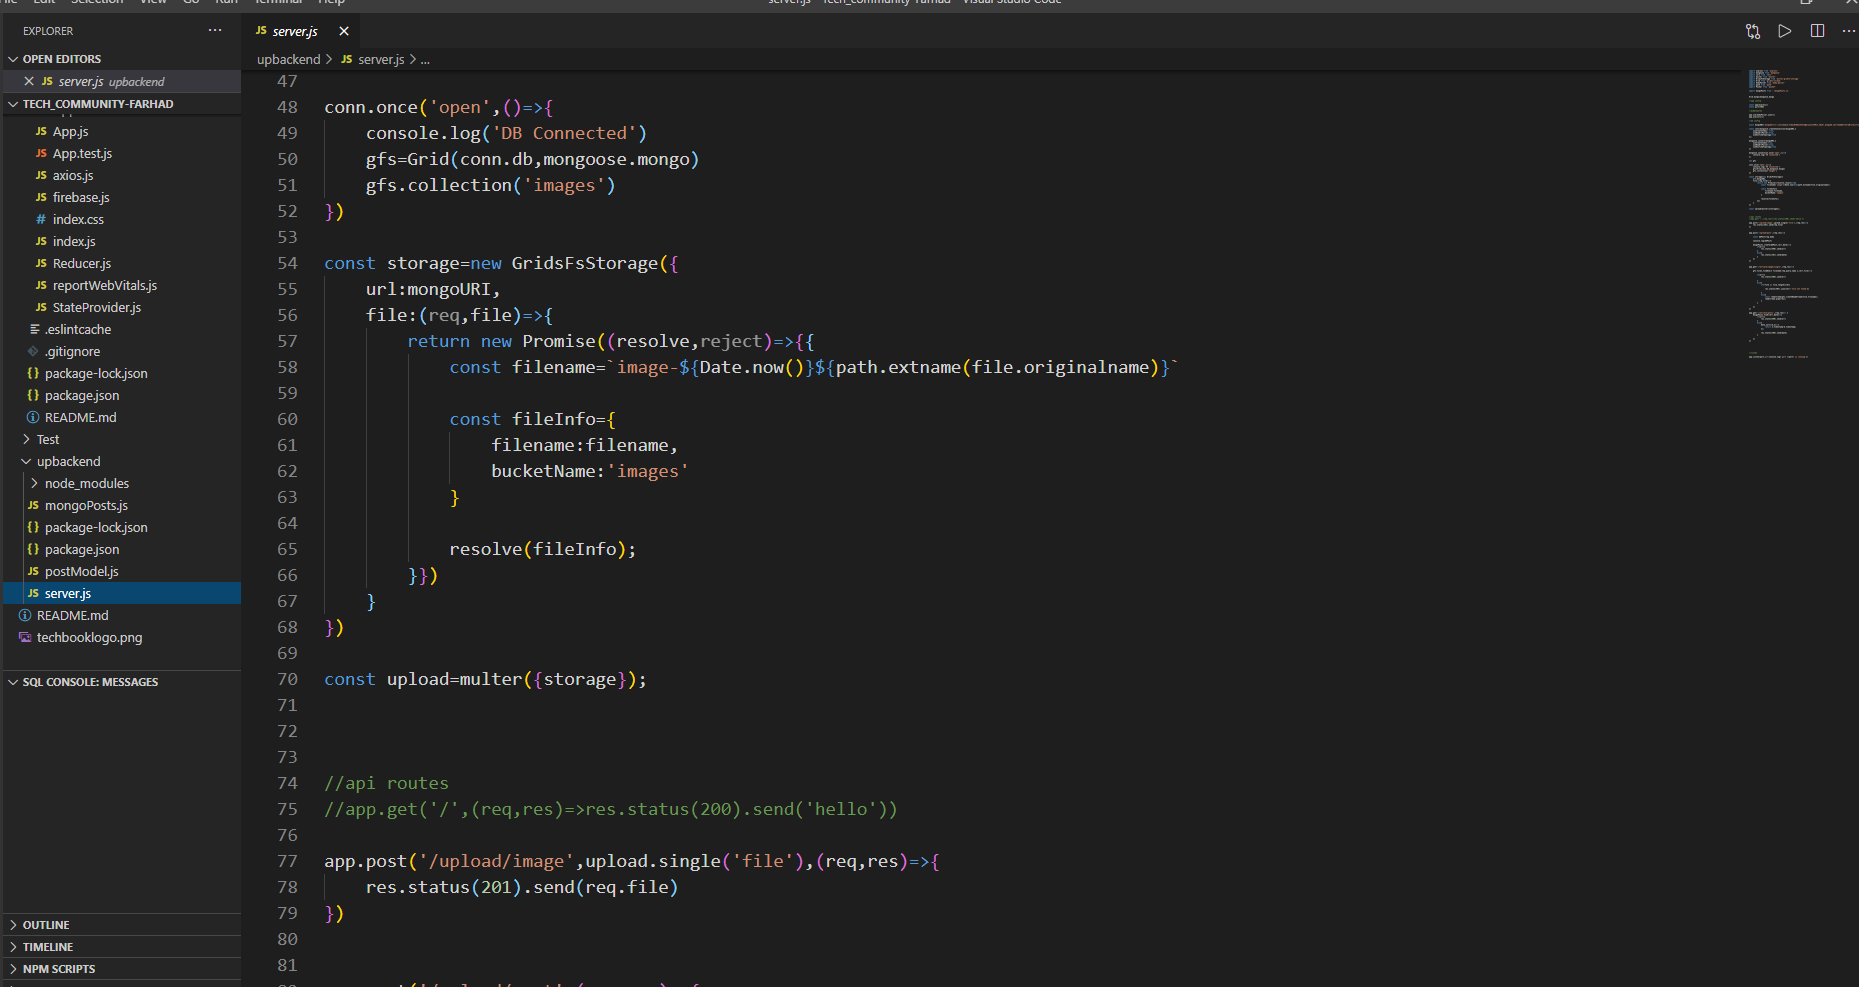
\includegraphics[scale=0.3]{./img/img5.png} 
\caption{Backend Coding Template}
 \label{fig:backend}
\end{figure}

\begin{figure}
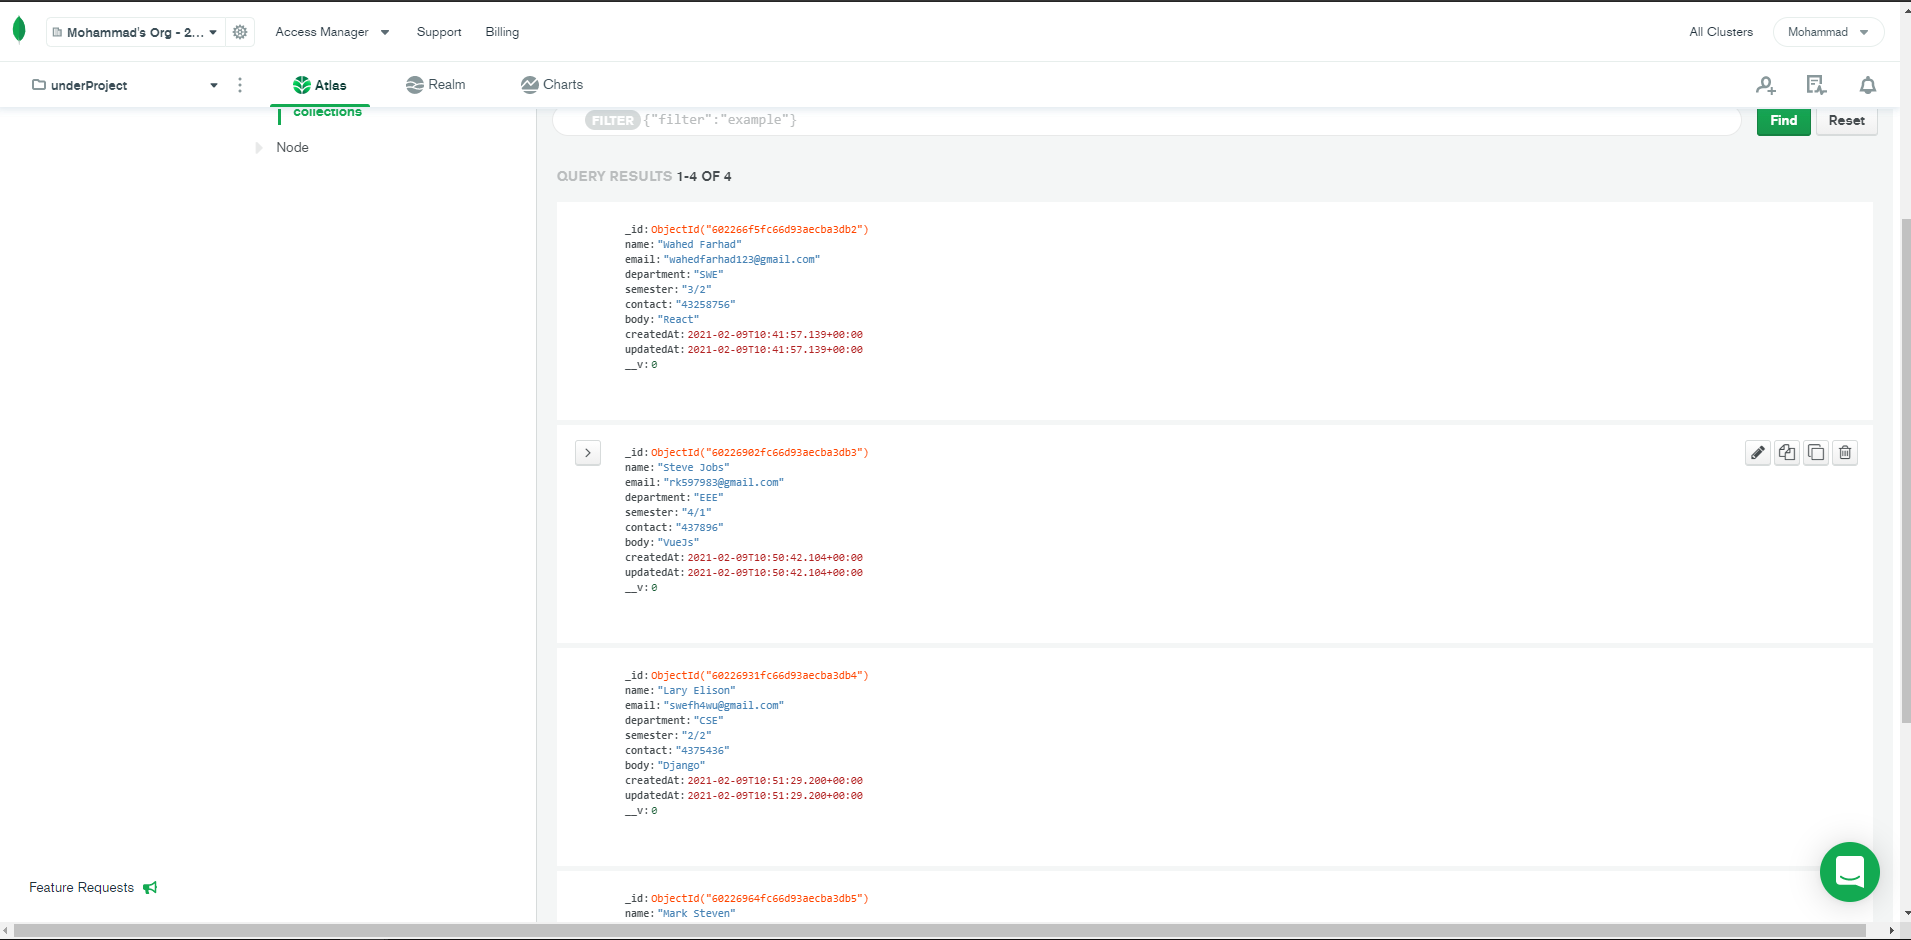
\includegraphics[scale=0.3]{./img/img4.png} 
\caption{MongoDB Template}
 \label{fig:DB}
\end{figure}

\clearpage
\vfill


%{\let\clearpage\relax\chapter*{5\hspace{0.3 cm} Resources}}
%\addcontentsline{toc}{chapter}{5\hspace{0.3 cm} Resources}

%For this platform we will use ReactJs for frontend and NodeJs for backend and also for database we use documented-oriented database like MongoDB.

%{\let\clearpage\relax\chapter*{6\hspace{0.3 cm} Conclusion}}
%\addcontentsline{toc}{chapter}{6\hspace{0.3 cm} Conclusion}

.

\end{document}